\documentclass{article}
\usepackage{graphicx} % Required for inserting images
\usepackage{todonotes}
\usepackage{url}
\usepackage{hyperref}
\title{Testing Techniques}
\author{Ivo Melse \& Marloes Bronsveld \& Madelief Slaats}
\date{September 2024}

\begin{document}
%\tiny % lol render eens zo
\small
\maketitle

\section*{Test Preparation: SUT Description}
\subsection*{1. Description of your SUT}
\subsubsection*{Synapse}
Our SUT is the server Synapse, which is open-source and the default and most complete Matrix homeserver. We will consider Synapse a black box, with interfaces through HTTP requests.

\subsubsection*{Functionality}
Synapse has quite a few functionalities, including the following.
\begin{itemize}
    \item Register/log in to an account
    \item Send messages/other types of media to other users
    \item Create/join chat-rooms 
    \item Connect with other Matrix homeservers
    \item End-to-End encryption
\end{itemize}
Since there are so many features, we will not focus on all of these in this assignment. We will focus on the Client-Server API, in particular on the functionality related to room membership.

\subsubsection*{External perspective}
The server communicates with the client through HTTP requests (see Figure \ref{fig:ext-per}). On receiving a request, the server will return a response. This might be an OK response or an error. Both requests and responses usually include a JSON file, in which information (for example, a message or error information) is stored.
\begin{figure}[h]
    \centering
    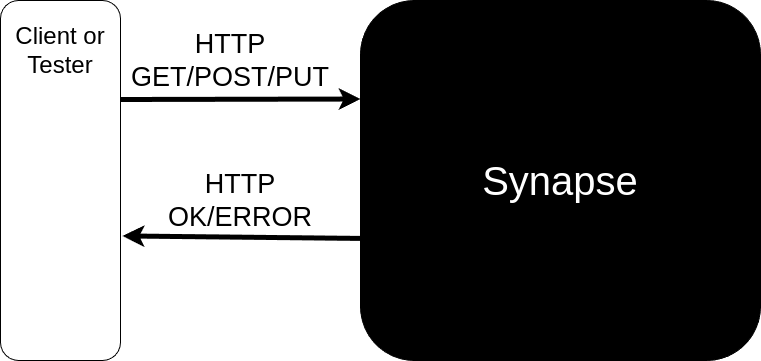
\includegraphics[width=0.5\linewidth]{External_perspective.drawio.png}
    \caption{External perspective of Synapse}
    \label{fig:ext-per}
\end{figure}

\noindent The SUT can be started and stopped in various ways depending on the setup. In our case, this works by running and stopping docker containers.

% \begin{itemize}
    
%     \item Functionality: Users should be able to connect to the Synapse server using a Matrix client. Synapse should provide the communication services as described in b).
%     \item Interfaces:
%         \begin{itemize}
%             \item Client-Server API: This allows communication between Synapse and Matrix clients.
%             \item ...
%         \end{itemize}
%     \item Inputs:
%         \begin{itemize}
%             \item User credentials (password)
%             \item Messages from users.
%             \item Messages forwarded by other homeservers.
%         \end{itemize}
%     \item Outputs:
%         \begin{itemize}
%             \item Messages
%             \item Notifications
%         \end{itemize}
%     \item Environments:
%     \item How to start/stop the SUT:
% \end{itemize}

\subsubsection*{Internal perspective}
Synapse has a Client-Server API with which it communicates with the Matrix Client. It presumably also communicates with an internal database that keeps track of the server state.

\begin{figure}[h]
    \centering
    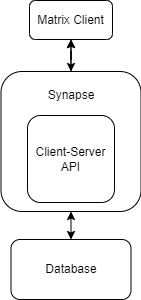
\includegraphics[width=0.18\linewidth]{internal_perspective.png}
    \caption{Internal perspective of Synapse}
    \label{fig:ext-per}
\end{figure}

\subsubsection*{Our setup}
Like aforementioned, we run Synapse using a docker container. Here is some more detailed information on our setup.
\begin{itemize}
    \item Ubuntu 24.04.1 LTS
    \item Docker version 27.3.1, build ce12230
    \item The latest Synapse version (1 October 2024)
\end{itemize}

\subsubsection*{Synapse and Client-server API documentation}
\begin{itemize}
    \item \href{https://github.com/matrix-org/synapse}{Synapse}
    \item \href{https://spec.matrix.org/latest/client-server-api/}{Client-Server API}
    \item \href{https://uhoreg.gitlab.io/matrix-tutorial/}{Simple client implementation in Python}
\end{itemize}

\subsection*{2. Quality aspects that matter for your SUT}
\subsubsection*{Quality characteristics}
\begin{enumerate}
    \item Reliability: Communication of clients via the Synapse server must be reliable. Messages should be synchronised and should not get `lost'.
    \item Security: The communication should be secure. Make sure that attackers cannot easily get access to information.
    \item Scalability: Synapse should be able to support a high amount of users.
\end{enumerate}


\subsubsection*{Related risks}
\begin{enumerate}
    \item Risk of failures: Failures in the system could cause downtime that impact people that rely on it for communication. It could also lead to data loss or integrity.
    \item Security: Lack of security could cause attackers to obtain valuable information from the users of the system.
    \item Performance issues: With scalability as an important quality characteristic, the system should be able to handle large amounts of users. This creates risks of overloading it which can lead to poor performance of the core functionalities.
\end{enumerate}
\subsubsection*{Quality assessment}
\begin{enumerate}
    \item White-box testing: Additionally to black-box testing, white-box testing can be a very effective way to test the system, by accessing the source code and using it to identify possible problematic parts of the system and test those extensively 
    \item Security testing: This is an important quality assessment, as security if a very important part of any messaging server. We can test how well Synapse is protected against attacks, for instance by looking at the end-to-end encryption, to ensure the safety of user data. 
    \item Usability testing: This is useful as an additional quality assessment to measure if the system can actually be used and managed in the way it was intended, and to see if the user experience is good.
\end{enumerate}

\section*{Test Preparation: Test Goal}
\subsection*{3. What are you going to test, on a global level?}
\subsubsection*{Focus}
We will test the API functionality related to room membership. We will consider this our main feature of focus.
We also have some test cases related to permissions, since this is a related feature.
Together these include joining rooms, leaving rooms, kicking and banning users.

\subsubsection*{Properties \& behaviour}
Relevant properties include room existence, membership, being invited to a room, and having permissions to perform administrative actions within a room. The behaviour that is relevant to us is concerned with changing these properties (server state).

\subsection*{4. The requirements/specification of the SUT}
We provide a short summary of the tested functionality. For more details (in particular about requests), we refer to the \href{https://spec.matrix.org/latest/client-server-api/#joining-rooms}{Matrix Client-Server API}.

A room can be public (anyone can join), trusted private (only invitees can join and will receive all admin privileges on joining), or private (only invitees can join).
If a user wishes to join a private room to which they are not invited, they can \textit{knock} on the room. 
Each member of a room has a \textit{power level} (by default 0-100). Power levels are Matrix' way of regulating permissions; 
The higher one's power level, the more administrative actions one can perform. Examples of actions that require a power level higher than 0 by default are kicking a user (the user is removed from a room) and banning a user (the user is kicked and is not able to join the room again). A user that has been banned can also be unbanned.
Rooms may have a join condition. If this is the case, only users who fulfill some extra requirement can join the room. 
At the time of writing this, the only join condition that is supported is membership of another room. A room can also be redirected to a new room. The old room is then archived and new users cannot join it. If a user does try to join, they will be redirected to the new room. Users that were in the old room can still inspect it, but if they want to send messages they should join the new room. You can also leave rooms, after which you should not be able to send and receive message from after they left. They also can't rejoin the room if it was a private room, and if they left before joining a private room the invite will be retracted.

\section*{Test Preparation: Test Method}
\subsection*{5. Provide a test architecture}
% \subsubsection*{a) give a diagram in which you position the SUT, its (distributed) structure, interfaces, environment, stubs, drivers, necessary test tools, . . . ;}
Our test setup is quite simple; we have an instance of the SUT and an instance of Postman, and a manual tester (a person). Using Postman, the manual tester sends requests to the server that mimic the behaviour of one or multiple clients. The tester observes the server's responses and verifies if they match the documentation of the Client-Server API.

\noindent See Figure \ref{fig:testing}.
\begin{figure}[h]
    \centering
    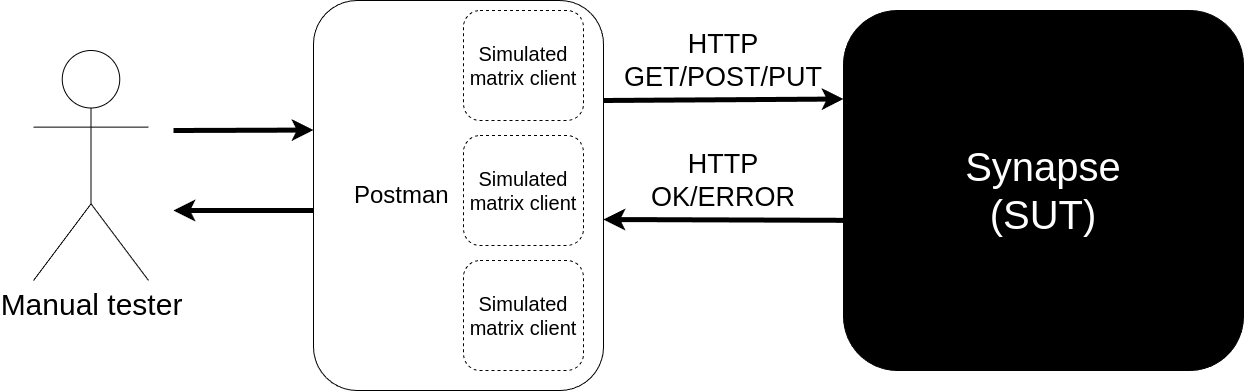
\includegraphics[width=0.8\linewidth]{Testing.drawio.png}
    \caption{An overview of the testing setup}
    \label{fig:testing}
\end{figure}

\noindent We run a Synapse server using docker, by running a container based on the image \href{https://hub.docker.com/r/matrixdotorg/}{synapsematrixdotorg/synapse}. We sent all requests to the default port 8008 on localhost. For simplicity, we will only use HTTP and not HTTPS.

Regarding the environment of the SUT, we assume that the server has enough available memory and a stable HTTP connection with the tester.
% \subsubsection*{b) describe the SUT input interfaces that you will use, i.e., where and how will your tests will trigger the SUT;}
% ...
% \subsubsection*{c) describe the SUT output interfaces, i.e., where and what you will observe during testing;}
% ...
% \subsubsection*{d) describe assumptions on the environment of the SUT;}
% ...
% \subsubsection*{e) describe which tools, stubs, drivers, . . . , you need for testing, consistent with the diagram that you made above.}
% ...

\subsection*{6. How will a typical test case look like:}
\subsubsection*{Test structure}
We consider our SUT to be in the initial state if the following holds.
\begin{itemize}
    \item The SUT (docker container) has just started running.
    \item There are three existing user accounts on the server: `one' with password `one', `two' with password `two', and `three' with password `three'.
    \item For the aforementioned accounts, we have a valid session. The session tokens are stored by the client.
    \item The default \texttt{homeserver.yaml} config file is used, 
    except that \texttt{enable\_registration: true} and 
    \texttt{enable\_registration\_without\_verification: true} are 
    added.
\end{itemize}

\noindent A test case follows the following structure. 
\begin{enumerate}
    \item Go to the initial state. This can be done by restarting the server.
    \item Establish sessions for the clients used for this test case.
    \item Using these sessions, write a request that activates the SUT behaviour that we want to test for this test case.
    \item Observe (manuallyl) if the response is consistent with the Client-Server API documentation.
\end{enumerate}


\subsubsection*{Test case notation}
We write our test cases in detailed steps that are still abstract from our implementation using Postman.

\section*{Test Preparation: Test Implementation}
\subsection*{7. Implementation of the test architecture}
\subsubsection*{Input and output interfaces}
As aforementioned, the input and output interface is the HTTP connection on http://localhost:8008.
The inputs are requests sent to this address and the outputs are the http responses.
\subsubsection*{Driver and testing tool}
As our main and only testing tool we use Postman. We have a \textit{collection} (a group of related requests) for each test case. We also have an \textit{environment} where some variables are defined (Tokens, URLS, etc.). We handed in our test implementations as JSON files which you should be able to import into Postman.
% \subsubsection*{d) are all test interfaces in the architecture accessible?}
% ...

\section*{Manual Testing}
In this section we describe our test cases in detail, but still abstracted away from the exact implementation.

\subsection*{8. The test input and output domains}
The domain of both inputs and outputs are HTTP requests. They are communicated over \texttt{localhost:8008}. Inputs are considered valid if they adhere to the \href{https://www.w3.org/Protocols/}{HTTP specification}, and are sent to \texttt{localhost:8008}.
\subsection*{Test generation techniques}
We will be using mostly state-based test generation. This makes sense in our case because the \textit{state} of the server determines if a user is part of a room or not.

\subsection*{10. Ten black-box functionality test cases}
% \todo{TODO remove this when we're done implementing}
% \begin{enumerate}
%     \item Create room
%     \begin{enumerate}
%         \item join room
%         \item send messages to other users
%     \end{enumerate}
%     \item Create room invite-only (private chat)
%     \begin{enumerate}
%         \item join room if invited
%         \item join room if not invited
%     \end{enumerate}
%     \item Create room power-level
%     \begin{enumerate}
%         \item make user admin/ give them more power
%         \item test if power user can do stuff
%         \item test if non-power user cannot do that stuff
%     \end{enumerate}
%     \item Create room with condition on joining room such that some users can join and others not (without invite)
%     \item Delete room
%     \begin{enumerate}
%         \item Test if user can still join deleted room
%         \item test if users still in room, can still message each other even if technically room is deleted.
%     \end{enumerate}
%     \item Ban user in room
%     \begin{enumerate}
%         \item Try to ban user of same power
%         \item Try to ban user of lower power
%         \item test if banned user cannot rejoin room
%         \item test if banned user can send/receive messages
%     \end{enumerate}
%     \item Test unbanning of user
%     \item Leave room
%     \begin{enumerate}
%         \item Test if user that left can indeed not send/receive messages from the room
%     \end{enumerate}
%     \item Leave an invite-only room
%     \begin{enumerate}
%         \item check if the invite is retracted, so that user cannot rejoin with same invite
%     \end{enumerate}
%     \item Knocking on rooms
%     \begin{enumerate}
%         \item Check if users can let user that knocked in
%     \end{enumerate}
% \end{enumerate}

Refer to the Appendix for more detailed tests.

\subsubsection*{1. Creation, membership, messages}
We test the basic functionality of creating a room, joining and sending a message. This includes verifying that a room with the same alias cannot be created twice and verifying that a user can only send a message in a room if they are a member of said room. To this end, we use EP.

\subsubsection*{2. Private (invite-only) room}
We verify that it is impossible for a user to join a private room without receiving an invite, and that a user with an invite \textit{can} join. This is an application of EP.

\subsubsection*{3. Kicking users and permissions}
We verify that only users with a sufficient power level can perform certain administrative actions. To test this, we use kicking a user, which requires level 50. We perform BVA on this level by testing it with level 49.

\subsubsection*{4. Room with join conditions}
Test if a user can create a room with a condition such as the condition that the user must already be a member of another room. Test whether users that comply to this condition can join and whether users that do not comply can join (without an invite). This is a form of EP.

\subsubsection*{5. Redirect rooms}
Rooms can be redirected to new rooms, while the old room gets `tombstoned'. We test whether this is possible and if users that were not in the old room, can still join the old room after it is tombstoned. We also check if users that were already in the old room can still send messages. Then we test if all users can easily join the new room. This testing is a form of EP as we try one case and assume this is a representative of all room redirections.

\subsubsection*{6. Ban user in room}
We test if a user can be banned and if this user is indeed kicked from the room. Banned users should not be allowed to rejoin the room, even if they receive an invitation. We test if this is the case. This test is a form of EP as we test it for one user.

\subsubsection*{7. Unban user in room}
We test if a banned user can be unbanned from a room and regain their normal rights. This is again EP.

\subsubsection*{8. Leave a room}
Test if a user can leave a room, they should show up in the member list as membership: "leave". They also should not be able to send any new messages and should not be able to receive any message sent after they left.

\subsubsection*{9. Leave an invite-only room}
In an invite-only room, the original invite should be deleted if a user leaves a room for which they were invited. If they want to rejoin they should obtain a new invite. We test if this is the case.

\subsubsection*{10. Leaving before joining}
The user can leave an invite-only room before they join it. If they do so, the original invite should be retracted anyway, and they should not be able to join the room. 

\subsection*{12. Discussion of the test results}
Test cases 1, 2, 6, 7, 9 and 10 give exactly the results that we expected. However, cases 3, 4 and 5 and 8 fail.

In the case of 3, we set the power level of user 'two' to 50, which is exactly the power level needed to kick another user. However, 'two' is still not permitted to kick 'three'.

In the case of 4, we have rooms \texttt{lobby} and \texttt{hotel}, which are both public rooms. \texttt{hotel} has a join rule that only allows users that are already in \texttt{lobby} to join. However, any user is able to join the \texttt{hotel} room, without being in the \texttt{lobby}.

In the case of 5, we have an old room and a new room, which are both public rooms. We try to tombstone the old room and redirect to the new room. This means that new users should not be able to join the old room and should be redirected to the new room. However, new users are still able to join the old room and send messages.

In the case of 8, we have a room that the user left. They correctly show up with membership: "leave" when requesting the members of the room, but they are still able to send messages and receive messages from after they left. 

Our test cases provide a solid code coverage on the functionality of rooms. We test most functionalities of the rooms and the test cases indicate that the core functionalities are solid, but there are some discrepancies that we found. These seem to indicate bugs in Synapse, but they might also be caused by faulty test case implementation. There's also one functionality we wanted to test, namely knocking on rooms, and the associated options, but we were not able to get the test case working at all, the knocking on rooms itself as it gave us an error "unrecognised request". Because of this we don't get full coverage of the room functionalities, but apart from this we get a good coverage.

\pagebreak
\section*{Appendix: Detailed test cases}
\subsubsection*{1. Creation, membership, messages}
1) One: create a public room called \texttt{room10} with alias \texttt{room10}\\
2) One: Repeat 1. (Supposed to fail)\\
3) One: Send a message in \texttt{room10}\\
4) Two: Send a message in \texttt{room10} (Supposed to fail)\\
5) Two: Join \texttt{room10}\\
6) Two: Send a message in \texttt{room10}\\
7) One: Get all messages in \texttt{room10} (manually verify 3, 4, 6)
We use equivalence partitioning between 1 and 2, and 4 and 5, since a message can either be sent successfully or fail because the user is not in the room.

\subsubsection*{2. Private (invite-only) room}
1) One: create a private room called \texttt{private10} with alias \texttt{private10}\\
2) One: invite user `two' to \texttt{private10}\\
3) Two: join \texttt{private10}\\
4) Two: send a message in \texttt{private10}\\
5) Three: join room \texttt{private10} (Supposed to fail)\\
6) Three: send a message in \texttt{private10} (Supposed to fail)\\
7) One: Get all messages in \texttt{room10} (manually verify 4, 6)

\subsubsection*{3. Kicking users and permissions}
1) One: create a public room called \texttt{power10} with alias \texttt{power10}.\\
2) Two: Kick `one' from \texttt{power10} (supposed to fail)\\
3) Two: Join \texttt{power10}\\
4) Two: Kick `three' from \texttt{power10} (supposed to fail)\\
5) Three: Join \texttt{power10}\\
6) Three: Send a message in \texttt{power10}\\
7) Two: Kick `three' from \texttt{power10} (supposed to fail)\\
8) One: Set the power level of `two' to 49 (moderator).\\
9) Two: Kick `three' from \texttt{power10} (supposed to fail)\\
10) One: Set the power level of `two' to 49 (moderator).\\
11) Two: Kick `three' from \texttt{power10}\\
12) Three: Send a message in \texttt{power10} (Supposed to fail)\\
13) One: Get all messages in \texttt{power10} (manually verify 6, 12)

\subsubsection*{4. Room with join conditions}
1) One: Create a public room called \texttt{lobby}\\
2) One: Create a public room called \texttt{hotel}\\
3) One: Set the join rule for \texttt{hotel} to only allow users that are already members of \texttt{lobby}.\\
4) Two: join \texttt{hotel} (Supposed to fail)\\
5) Two: Send a message in \texttt{hotel} (Supposed to fail)\\
6) One: Get all messages in \texttt{hotel} (Manually verify 5)

\subsubsection*{5. Redirect rooms}
1) One: Create public room called \texttt{room50} \\
2) Two: Join \texttt{room50} \\
3) One: Create new public room called \texttt{room51} \\
4) One: Send tombstone message which redirects \texttt{room50} to \texttt{room51} \\
5) Three: Join \texttt{room50} (Should fail) \\
6) Three: Join \texttt{room51} \\
7) Two: Send message in \texttt{room50} (Should fail) \\
8) Two: Join \texttt{room51} \\
9) Two: Send message in \texttt{room51} \\
10) One: Get all messages in \texttt{room50} (Manually verify 7) 

\subsubsection*{6. Ban user in room}
1) One: Create a public room called \texttt{room60} with alias \texttt{room60}\\
2) Two: Join \texttt{room60} \\
3) Two: Send a message in \texttt{room60} \\
4) One: Ban `two' from \texttt{room60} \\
5) Two: Send a message in \texttt{room60} (Supposed to fail) \\
6) One: Send a message in \texttt{room60} \\
7) Two: Get all messages in \texttt{room60} (Supposed to fail) \\
8) Two: Join \texttt{room60} (Supposed to fail) \\
9) One: Invite `three' to \texttt{room60} \\
10) One: Invite `two' to \texttt{room60} (Supposed to fail) \\
11) One: Get all messages in \texttt{room60} (Manually verify 5)

\subsubsection*{7. Unban user in room}
1) One: Create a public room called \texttt{room70} with alias \texttt{room70}\\
2) Two: Join \texttt{room70} \\
3) One: Ban `two' from \texttt{room70} \\
4) Two: Send a message in \texttt{room70} (Supposed to fail) \\
5) One: Unban `two' from  \texttt{room70} \\
6)  Two: Send a message in \texttt{room70} (Supposed to fail) \\
7) Two: Join \texttt{room70} \\
8) Two: Send a message in \texttt{room70} \\
9) One: Get all messages in \texttt{room60} (Manually verify 4, 6)

\subsubsection*{8. Leave a room}
1) One: Create a public room called \texttt{room80} with alias \texttt{room80} \\
2) Two: Join \texttt{room80} \\
3) Two: Leave \texttt{room80} \\
4) One: Check members of room \texttt{room80} \\
5) Two: Send a message in room \texttt{room80} (Supposed to fail) \\
6) One: Send a message in room \texttt{room80} \\
7) Two: Get all message from \texttt{room80} (Supposed to not get the message from step 6) 

\subsubsection*{9. Leave an invite-only room}
1) One: Create a private room called \texttt{room90} with alias \texttt{room90} \\
2) One: Invite user 'two' to room \texttt{room90} \\
3) Two: Join room \texttt{room90} \\
4) Two: Leave room \texttt{room90} \\
5) One: Check members of room \texttt{room90} \\
6) Two: Join room \texttt{room90} again (Supposed to fail)

\subsubsection*{10. Leaving before joining}
1) One: Create a private room called \texttt{room100} with alias \texttt{room100} \\
2) One: Invite user 'two' to room \texttt{room100} \\
3) Two: Leave room \texttt{room100} \\
4) One: Check members of room \texttt{room100} \\
5) Two: Join room \texttt{room100} (Supposed to fail) \\
6) One: Check members of room \texttt{room100} 

\end{document}
